\chapter[CAPÍTULO I]{GENERALIDADES DE LA EMPRESA}

\section{Datos Generales de la Empresa}

\subsection{Reseña Histórica de la Empresa}
J\&P Periféricos S.A.C. es una empresa peruana del sector informático que inició sus operaciones el 1 de octubre del año 2011. Su propósito es brindar soluciones informáticas a empresas cuyas necesidades son la mejora de sus procesos internos. Asimismo, ofrece la venta de productos tecnológicos tanto a personas naturales como empresas.

Con el paso de los años, J\&P Periféricos fue logrando consolidar su presencia en el sector y especializando sus soluciones de acuerdo a las necesidades de sus clientes. Además, ha ampliado el alcance de sus servicios, dando mantenimiento y soporte técnico continuo con el fin de alcanzar una mayor credibilidad y mejorar la relación con sus clientes.

\subsection{Quiénes Somos}
J\&P Periféricos S.A.C. es una empresa peruana en el rubro de la informática que brinda soluciones integrales informáticas tales como el mantenimiento informático, venta de productos tecnológicos, desarrollo de páginas web, redes y comunicaciones, empleando tecnología actual para una mejor eficiencia y rapidez en sus procesos.

\subsection{Razón Social}
\noindent
\begin{tabular}{@{} p{3.2cm} p{4.5cm} p{2.5cm} p{5.5cm} @{}}
    \textbf{Nombre Empresa} & J\&P Periféricos S.A.C. & \textbf{Empresario} &Julio Flores Vicuña \\[0.5em]
    \textbf{Razón Social}   & 20545122520             & \textbf{Rúbrica}    & Soluciones Informática Cerrada \\[0.5em]
    \textbf{Distrito}       & Cercado de Lima         & \textbf{Dirección}  & \raggedright Jr. Emilio Fernández 160 Dpto. 1804 \\
\end{tabular}

\begin{figure}[H]
    \centering
    \captionsetup{justification=centering}
    \caption{Logotipo Institucional de J\&P Periféricos S.A.C.}
    \label{fig:logo_empresa}
    \vspace{0.4em}
    
    
\includegraphics[width=0.7\textwidth]{img/logo-empresa.png}
    
    \vspace{0.4em}
    {\small \textit{Nota.} Gráfico representativo del logotipo corporativo de la empresa.}
\end{figure}

\subsection{Localización de la Empresa}
La sede de \textbf{J\&P Periféricos S.A.C.} se encuentra ubicada en el departamento Concepto Urbano Plus, Calle Emilio Fernández 160, Dpto. 1804, distrito de Cercado de Lima (Código Postal 15046). Como referencia de acceso principal, el inmueble se ubica a la altura de la cuadra 8 de la Avenida Arequipa.

\begin{figure}[H] 
    \centering
    \captionsetup{justification=centering}
    \caption{Localización y vías de acceso de la empresa}
    \label{fig:mapa_ubicacion}
    \vspace{0.4em}
    
    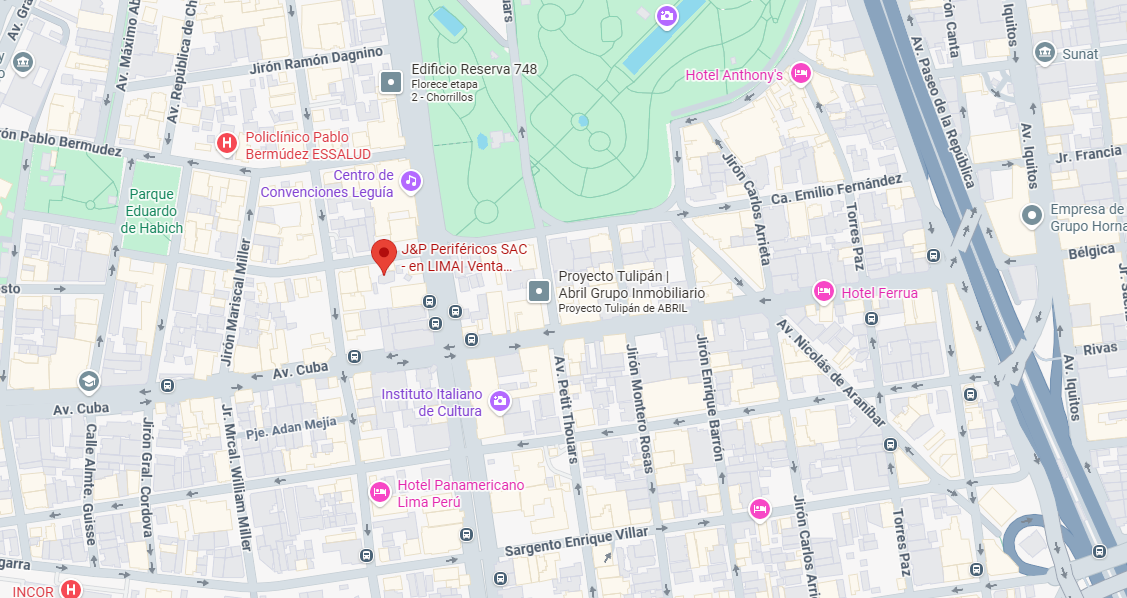
\includegraphics[width=0.8\textwidth]{img/direccion-empres.png}
    
    \vspace{0.4em}
    {\small \textit{Nota.} Ubicación geográfica y mapa vial de la sede central. Adaptado de Google Maps.}
\end{figure}

\FloatBarrier

\section{Misión, Visión, Objetivos y Valores de la Empresa}

\subsection{Misión}
Proporcionar soluciones tecnológicas orientadas a la optimización de los procesos de negocio, facilitando a los clientes métodos efectivos para afrontar los desafíos informáticos empresariales mediante la implementación estratégica y adecuada de las tecnologías de la información.

\subsection{Visión}
Posicionarse como una organización referente en soluciones informáticas, altamente eficiente y rentable, operando bajo estándares de calidad internacional, con un equipo humano calificado y un firme compromiso con el desarrollo sostenible y la preservación del medio ambiente, garantizando la expansión y continuidad del negocio.

\subsection{Objetivos}
% Objetivos a corto plazo
\noindent\textbf{Objetivos a Corto Plazo:}
\begin{itemize}
    \item Consolidar la presencia y posicionamiento comercial en el mercado peruano.
    \item Ampliar la cartera de clientes corporativos e individuales.
    \item Diversificar y actualizar el portafolio de servicios tecnológicos.
    \item Incrementar los índices de satisfacción y fidelización de los clientes.
    \item Optimizar los flujos operativos y tiempos de respuesta en los procesos internos.
\end{itemize}

% Objetivos a largo plazo

\noindent\textbf{Objetivos a Largo Plazo:}
\begin{itemize}
    \item Posicionarse como una empresa líder e innovadora en el sector de tecnologías de la información.
    \item Asegurar la sostenibilidad financiera y la escalabilidad operativa del modelo de negocio.
    \item Contribuir activamente a la transformación digital y al desarrollo tecnológico nacional.
\end{itemize}

\subsection{Valores de la Empresa}
\begin{itemize}
    \item \textbf{Orientación al cliente:} Atención focalizada en los requerimientos específicos de cada cliente, diseñando soluciones a medida que potencien sus procesos de negocio.
    \item \textbf{Innovación continua:} Adopción y aplicación proactiva de tecnologías emergentes para generar valor agregado y dinamismo operativo.
    \item \textbf{Calidad y excelencia:} Compromiso con la entrega de productos y servicios que cumplan con altos estándares técnicos y de rendimiento.
    \item \textbf{Desarrollo humano:} Fomento del crecimiento profesional, técnico y personal del capital humano como pilar del éxito organizacional.
    \item \textbf{Responsabilidad social y ambiental:} Conciencia ambiental y ética corporativa orientada al desarrollo sostenible y buenas prácticas operativas.
\end{itemize}

\section{Producto, Mercado y Cliente}

\subsection{Producto}
La empresa \textbf{J\&P Periféricos S.A.C.} comercializa una gama integral de equipamiento informático, 
suministros y soluciones tecnológicas orientadas tanto al usuario final como al sector corporativo de Lima Metropolitana. Su portafolio de productos y servicios incluye:

\begin{itemize}
    \item \textbf{Laptops y Tablets:} Equipos portátiles para uso personal, profesional y entornos de alto rendimiento.
    \item \textbf{PC y Servidores:} Computadoras de escritorio ensambladas a medida y estaciones de trabajo o servidores para infraestructura empresarial.
    \item \textbf{Impresoras:} Equipos de impresión multifuncionales, térmicos y de inyección o láser para oficina.
    \item \textbf{Monitores:} Pantallas y soluciones de visualización con diversas resoluciones y tecnologías de panel.
    \item \textbf{Componentes para PC:} Placas base, procesadores, memorias, tarjetas de video y unidades de almacenamiento en estado sólido.
    \item \textbf{Accesorios y Repuestos:} Periféricos de entrada/salida, cables estructurados, fuentes de poder y partes de recambio.
    \item \textbf{Soluciones Corporativas:} Servicios de integración tecnológica, mantenimiento preventivo/correctivo y soporte continuo de infraestructura TI.
\end{itemize}

Como parte de la diversificación de su portafolio tecnológico, J\&P Periféricos S.A.C. ha impulsado el desarrollo de un sistema web centralizado para la gestión integral de mesas de ayuda (Help-Desk), control de inventario de activos TI (ITAM) y automatización de soporte técnico presencial y remoto. La empresa proyecta ofrecer esta solución a sus clientes corporativos bajo un modelo modular de servicios tecnológicos. El presente proyecto comprende el desarrollo, despliegue y validación de esta solución en la propia organización; su comercialización externa se plantea como una etapa posterior.

\subsection{Mercado}
El mercado objetivo de la organización se enmarca dentro del sector de las Tecnologías de la Información y Comunicación (TIC). La oferta está dirigida principalmente al segmento empresarial (B2B) y a profesionales independientes (B2C) en Lima Metropolitana que requieren aprovisionamiento de hardware, despliegue de redes, mantenimiento de infraestructura informática y optimización técnica de sus procesos de negocio mediante herramientas digitales.

Para el producto desarrollado en este proyecto, los destinatarios previstos son empresas que requieren integrar la información laboral de sus trabajadores con el procesamiento de nóminas, la revisión de incidencias y la generación de documentos. La cartera existente constituye un ámbito potencial para identificar usuarios interesados, sin que ello implique que todos sus integrantes hayan solicitado o contratado la solución.

\subsection{Cliente}
La cartera de clientes de \textbf{J\&P Periféricos S.A.C.} abarca diversas entidades comerciales, industriales, de salud y servicios profesionales, entre las cuales destacan:

\begin{itemize}
    \item Grupo Enfoque
    \item Sergetic
    \item S\&R Solution Service
    \item Hidromax S.A.C.
    \item Copaco S.A.C.
    \item Fasetron del Perú S.A.C.
    \item Asociación Peruana de Nefrología Pediátrica
    \item Distribuidora Venso S.A.C.
    \item Textiles TBM S.A.C.
\end{itemize}

\section{Organigrama de la Empresa}

\begin{figure}[H]
    \centering
    \captionsetup{justification=centering}
    \caption{Estructura orgánica funcional de J\&P Periféricos S.A.C.}
    \label{fig:organigrama_empresa}
    \vspace{0.2em}
    
    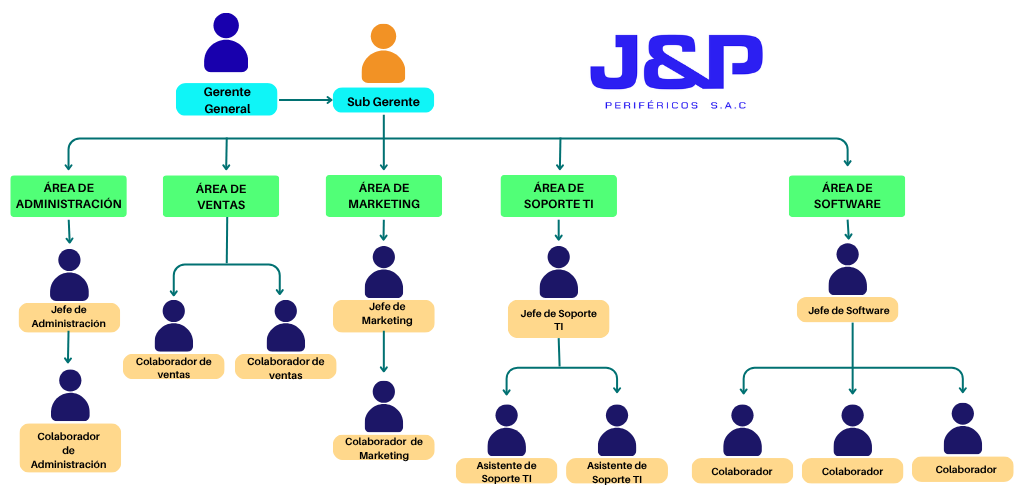
\includegraphics[width=1.0\textwidth]{img/organigrama_empresa.png}
    
    \vspace{0.2em}
    {\small \textit{Nota.} Representación jerárquica y departamental de las áreas funcionales de la empresa. Elaboración propia.}
\end{figure}

\clearpage

\section{Otra Información Relevante de la Empresa donde se desarrolla el Proyecto}

\subsection{Planificación y Gestión de la Entrevista}
Con el propósito de profundizar en el diagnóstico situacional, contrastar la perspectiva estratégica del negocio y sustentar las causas raíz de las deficiencias operativas en la atención de soporte técnico y el control de inventario de activos TI, se diseñó e implementó una entrevista semiestructurada aplicada a los responsables directos de la gestión empresarial y del área de tecnología.

\vspace{0.3cm}
\noindent\textbf{Entrevistado:} Julio Flores Vicuña, \textbf{Gerente General de J\&P Periféricos S.A.C.}
\vspace{0.4cm}

\begin{enumerate}[leftmargin=*, label=\textbf{P\arabic*.}]
    \item \textbf{¿Cuáles son las principales dificultades de gestión interna que ha identificado en la atención de soporte técnico e inventario de TI?}
    
    \textit{Respuesta del Gerente General:} La falta de un canal centralizado de atención. Las solicitudes ingresan por WhatsApp o llamadas informales, lo que genera desorden, solicitudes traspapeladas, retrasos en la respuesta y la imposibilidad de saber qué equipos o licencias tiene asignados cada cliente.

    \item \textbf{¿Qué motivos estratégicos llevaron a la empresa a optar por el desarrollo de un sistema Help-Desk propio en lugar de contratar un software comercial?}
    
    \textit{Respuesta del Gerente General:} Requerimos una solución adaptada a nuestro modelo de negocio multinivel, que integre en una sola plataforma la gestión de tickets, la programación de visitas técnicas in-situ, el control de planes/contratos de soporte y el inventario detallado de hardware y software por cliente.

    \item \textbf{Desde su perspectiva gerencial, ¿cuáles representan los mayores desafíos al momento de supervisar al personal técnico y los servicios prestados?}
    
    \textit{Respuesta del Gerente General:} La ausencia de indicadores de rendimiento (KPIs) en tiempo real. Sin métricas como el tiempo medio de respuesta (MTTA) o resolución (MTTR), es muy difícil evaluar el desempeño de los técnicos y garantizar el cumplimiento de los Acuerdos de Nivel de Servicio (SLA).

    \item \textbf{¿Qué impacto operativo y económico espera que genere la implementación de este sistema Help-Desk?}
    
    \textit{Respuesta del Gerente General:} En lo operativo, estandarizará la atención y eliminará los cruces de horario en las visitas técnicas. En lo económico, reduciremos costos por desplazamientos ineficientes y mejoraremos la retención de clientes corporativos al brindar un servicio transparente y medible.

    \item \textbf{¿Qué necesidades comunes comparten las empresas de su cartera a las que estará orientada la plataforma?}
    
    \textit{Respuesta del Gerente General:} Todas las empresas cliente necesitan trazabilidad sobre las fallas de sus equipos, conocer el historial de mantenimientos y tener la certeza de que sus incidencias críticas se atienden dentro de los tiempos contratados.
\end{enumerate}

\vspace{0.3cm}
\noindent\textbf{Entrevistado:} Jack Huaman, \textbf{Jefe de Soporte Técnico y TI de J\&P Periféricos S.A.C.}
\vspace{0.4cm}

\begin{enumerate}[leftmargin=*, label=\textbf{P\arabic*.}]
    \item \textbf{¿Cuánto tiempo promedio invierte diariamente el equipo en clasificar, asignar y dar seguimiento manual a las solicitudes de soporte?}
    
    \textit{Respuesta del Jefe de TI:} Aproximadamente entre 2 a 3 horas diarias coordinando por mensajes o llamadas, consolidando datos en hojas de cálculo y preguntando al cliente datos básicos del equipo afectado antes de iniciar el diagnóstico.

    \item \textbf{¿Cuáles son los principales cuellos de botella que se presentan al atender un requerimiento sin una base de datos de activos unificada?}
    
    \textit{Respuesta del Jefe de TI:} La falta de antecedentes técnicos. Muchas veces los técnicos van a atender a ciegas sin conocer la configuración, garantías o historial de reparaciones previas del hardware, lo que ocasiona diagnósticos repetitivos y reescritura de informes.

    \item \textbf{¿Cómo se gestiona actualmente la programación de visitas presenciales in-situ y qué problemas ocasiona?}
    
    \textit{Respuesta del Jefe de TI:} Se realiza de forma empírica y verbal. Generando de vez en cuando cruces de horario entre los técnicos, traslados duplicados a la misma zona o demoras en la llegada a clientes con incidencias de prioridad alta.

    \item \textbf{¿Qué errores o inconsistencias son más frecuentes al controlar los contratos y el inventario mediante hojas de cálculo?}
    
    \textit{Respuesta del Jefe de TI:} El desequilibrio de información. Con frecuencia se prestan servicios a equipos que ya no están cubiertos por el plan del cliente o no se registran los componentes o repuestos reemplazados durante la atención.

    \item \textbf{¿Qué herramientas o métricas considera indispensables en el nuevo sistema web?}
    
    \textit{Respuesta del Jefe de TI:} Un panel de tickets por estado y prioridad, un expediente técnico digital por cada activo informático, un calendario de rutas/citas in-situ y un tablero de control con métricas como el tiempo de solución y la satisfacción del cliente.
\end{enumerate}